\section{Experiments}
\label{sec:experiments}
We evaluate ACRO across pretrained policies, simulated environments, and a real robot. Section~\ref{sec:main_results} examines its use across these execution settings and the data needed to prepare the Critic. Section~\ref{sec:analysis} studies Critic-guided recovery and the efficiency of execution after returning. Section~\ref{sec:data-retraction} examines test-time scaling and physical return cost. Appendix~\ref{sec:ablations} examines Critic architectures and intervention triggers.

\Needspace{9\baselineskip}
\subsection{Experimental Setup}
\label{sec:exp_setup}

\paragraph{Models and Datasets.}
We use two pretrained VLAs with their policies fixed throughout execution: GR00T N1.7~\citep{nvidia2026groot17} on SimplerEnv Bridge~\citep{li2025simpler}, and $\pi_{0.5}$~\citep{black2025pi05} on RoboCasa~\citep{nasiriany2024robocasa}. SimplerEnv Bridge tests fine-grained tabletop manipulation, while RoboCasa covers a broader range of household object interactions. We also evaluate $\pi_{0.5}$ on a real robot to test recovery under physical sensing and actuation conditions. \Cref{fig:environments} introduces the three evaluation environments.
\begin{figure}[!t]
  \centering
  \begin{minipage}{0.88\linewidth}
    \captionsetup[subfigure]{font=small,skip=4pt,justification=centering}
    \begin{subfigure}{\linewidth}
      \centering
      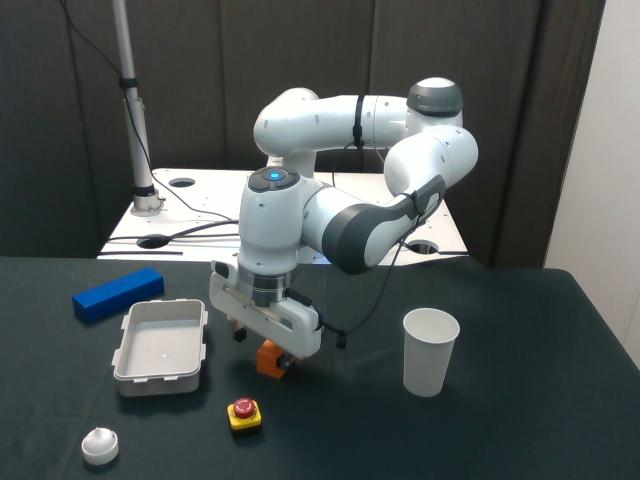
\includegraphics[width=0.326\linewidth]{assets/real_robot/panda_pick/front_059.jpg}\hfill
      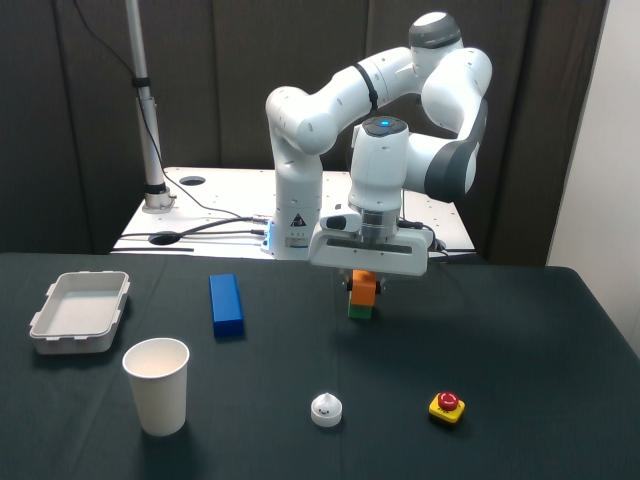
\includegraphics[width=0.326\linewidth]{assets/real_robot/cube_stack/front_011.jpg}\hfill
      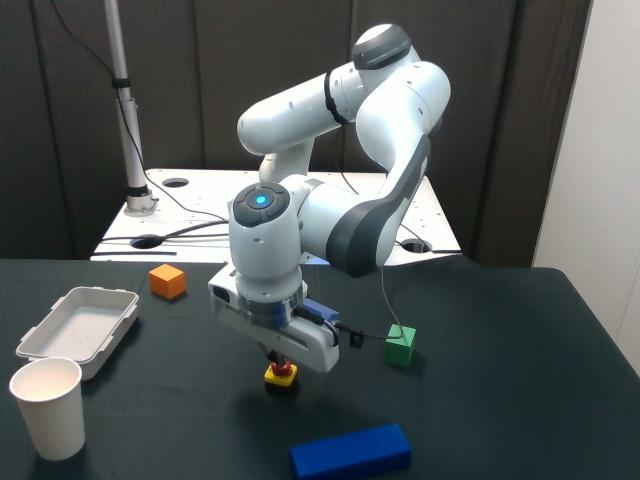
\includegraphics[width=0.326\linewidth]{assets/real_robot/press_button/front_010.jpg}
      \caption{Real Robot}
      \label{fig:environments-real}
    \end{subfigure}

    \medskip
    \begin{subfigure}[t]{0.482\linewidth}
      \centering

      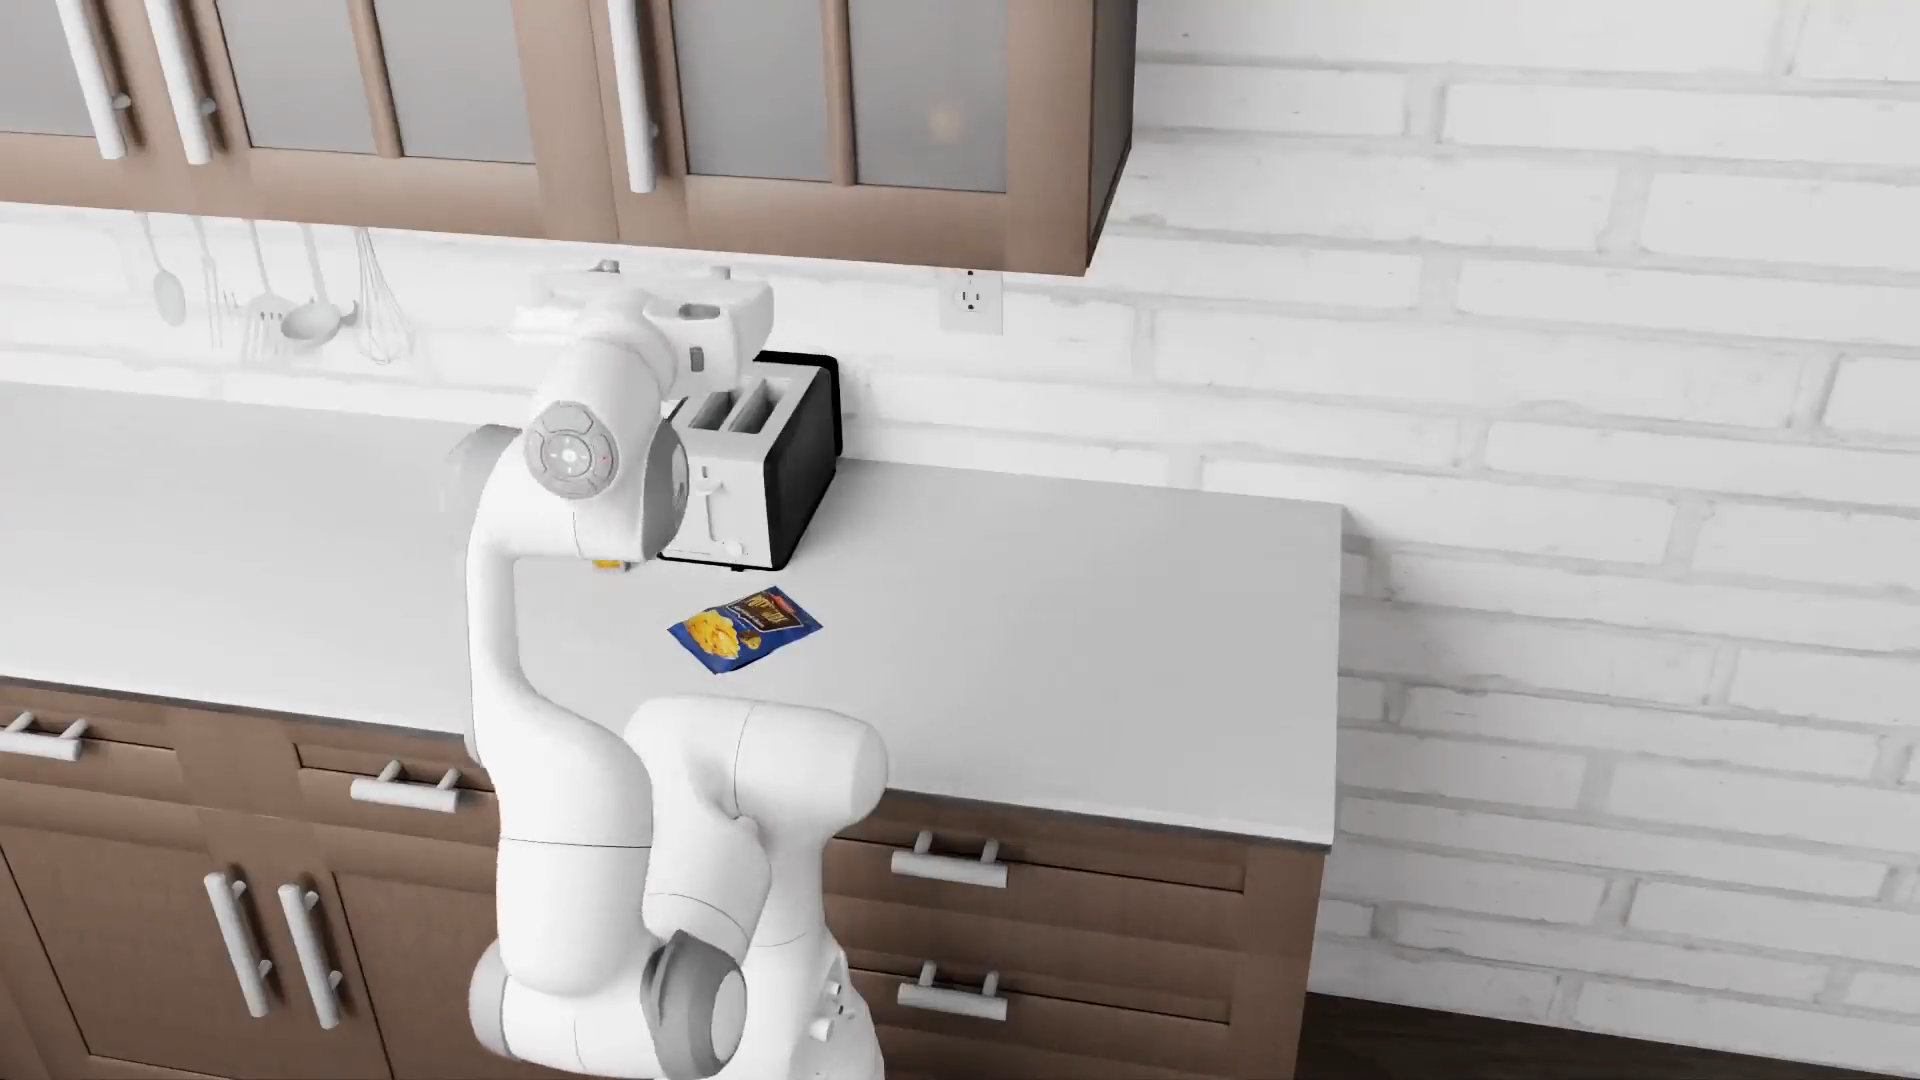
\includegraphics[width=0.489\linewidth,trim={240 0 240 0},clip]{assets/environments/robocasa.png}\hfill
      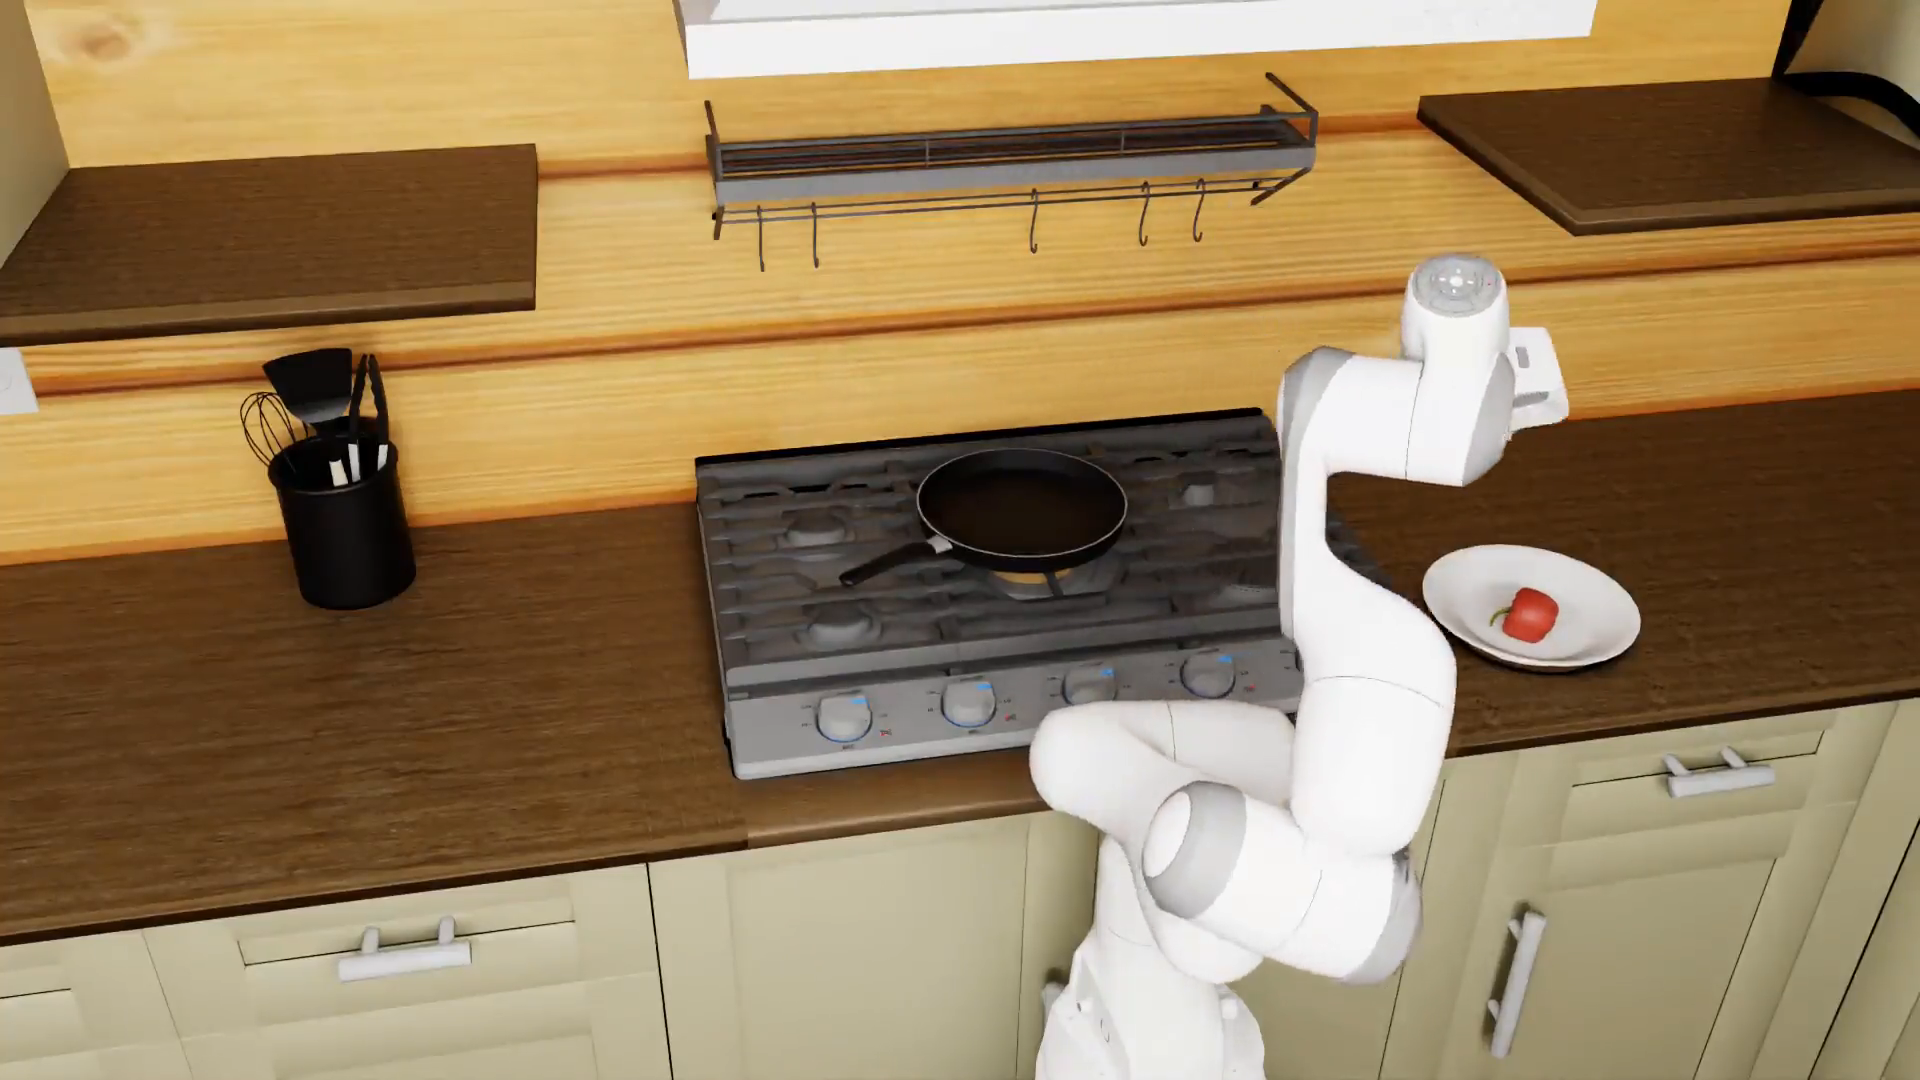
\includegraphics[width=0.489\linewidth,trim={350 0 130 0},clip]{assets/environments/robocasa-pnp.png}
      \caption{RoboCasa}
      \label{fig:environments-robocasa}
    \end{subfigure}\hfill
    \begin{subfigure}[t]{0.482\linewidth}
      \centering

      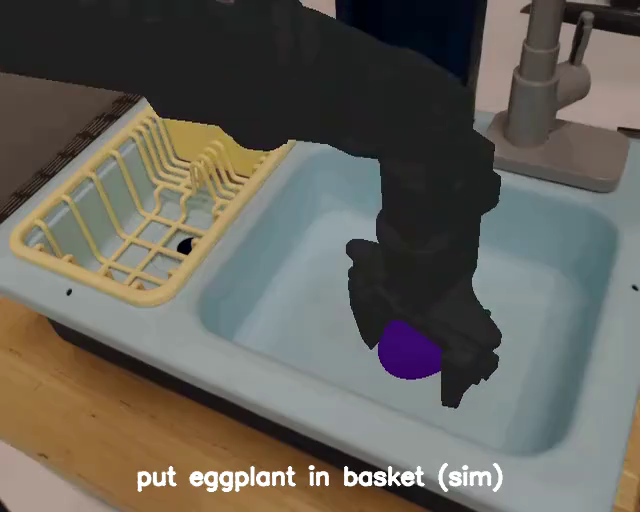
\includegraphics[width=0.489\linewidth,trim={20 62 20 0},clip]{assets/environments/bridge.png}\hfill
      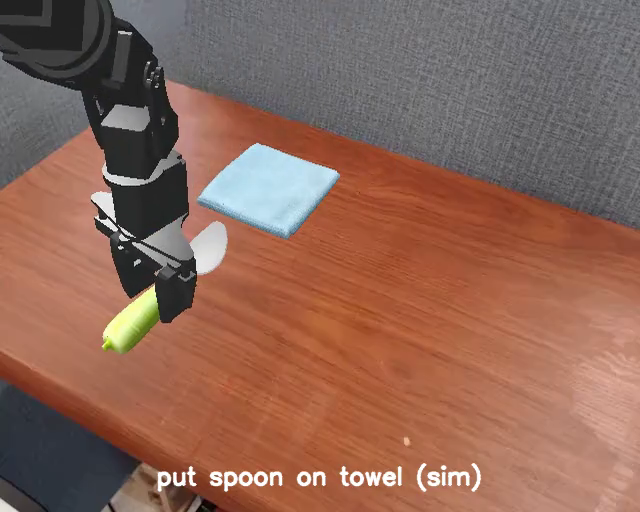
\includegraphics[width=0.489\linewidth,trim={20 62 20 0},clip]{assets/environments/bridge-spoon.png}
      \caption{SimplerEnv Bridge}
      \label{fig:environments-bridge}
    \end{subfigure}
  \end{minipage}
  \caption{Evaluation environments. (a) Real robot: pick and place, cube stacking, and button pressing. (b) RoboCasa~\citep{nasiriany2024robocasa}: cabinet interaction and pick and place. (c) SimplerEnv Bridge~\citep{li2025simpler}: eggplant in basket and spoon on towel. Scenes are ordered left to right within each group; simulation images are from official project demonstrations.}
  \label{fig:environments}
\end{figure}


\paragraph{Baselines.}
We compare three ways of using the execution budget: uninterrupted policy execution, value-ranked action selection, and recovery through physical repositioning. Base VLA executes the underlying policy without intervention. RoboMonkey~\citep{kwok2025robomonkey} selects among candidate actions at the current state. Our adaptation uses ACRO's Q estimate as its verifier to rank eight action chunks at each policy query. This compares using the same Critic for action selection with using it to guide ACRO's interventions, while requiring eight policy samples per query. CycleVLA~\citep{ma2026cyclevla} uses a VLM to decompose the instruction into subtasks, check completion at subtask boundaries, and return the robot to the start of a failed subtask before retrying. This provides a comparison with recovery guided by an external VLM. Our adaptation keeps the base policy fixed and omits the original policy fine-tuning. On RoboCasa, Periodic rewind provides a fixed-schedule recovery baseline: it returns along the recorded path at fixed intervals to a fixed look-back distance. For real-robot experiments, we compare ACRO with Base VLA. \Cref{app:details} gives the implementation details of all methods.

\paragraph{Implementation Details.}
For a fair comparison, all methods use the same evaluation identities and receive the same physical step budget, which includes intervention motion. Additional policy and VLM queries do not count toward this physical step budget. We use each benchmark's standard episode limit: 300 steps on SimplerEnv, the official GR00T evaluation limit, and each task's registered limit on RoboCasa. To learn when and where to intervene, we train the Critic on uninterrupted rollouts of the base policy (1230 on SimplerEnv and 1200 on RoboCasa) using AdamW with a learning rate of $10^{-3}$, and set the intervention threshold by calibrating on held-out rollouts so that about 20\% of executions that would succeed raise an alarm. We measure task success over 240 trials on SimplerEnv, 600 on RoboCasa, and 60 on the real robot, pooling trials within each environment for overall performance. The scheduled-rewind and outcome analyses reuse all 600 RoboCasa evaluation trials at the same standard physical budget $H$. For the separate Critic and path ablations, we use $\pi_{0.5}$ on three RoboCasa tasks, one from each category: Turn On Electric Kettle (Control), Open Stand Mixer Head (Open), and Pick-and-Place Counter to Cabinet (Pick and Place).
